\documentclass[12pt, a4paper]{article}

% Preamble: Essential packages
\usepackage[margin=2.5cm]{geometry}
\usepackage{amsmath}
\usepackage{amssymb}
\usepackage{graphicx}
\usepackage{tikz}
\usepackage{microtype} % For better typesetting
\usepackage{fontawesome5} % For rocket icon
\usepackage{hyperref}
\hypersetup{
    colorlinks=true,
    linkcolor=blue,
    filecolor=magenta,      
    urlcolor=cyan,
}

% TikZ library for arrows and intersections
\usetikzlibrary{arrows.meta, intersections}

% Title setup
\title{New Problems in Special Relativity: A Self-Study Guide}
\author{}
\date{\today}

\begin{document}
\maketitle
\tableofcontents
\newpage

\section{New Problems and Solutions}

\subsection{Problem 1: The Journey to Proxima Centauri}
\textbf{Question:} \textit{An advanced interstellar probe is sent on a mission to Proxima Centauri, located 4.2 light-years away from Earth as measured by astronomers on Earth. The probe travels at a constant velocity of 0.7c.}
\vspace{1em}

\textbf{(a)} \textit{How long does the journey take according to mission control on Earth?}
\vspace{1em}
This is a simple time, distance, and speed calculation in the Earth's reference frame.
Distance $d = 4.2 \text{ light-years} = 4.2c \cdot \text{years}$. Velocity $v = 0.7c$.
$$t = \frac{d}{v} = \frac{4.2c \cdot \text{years}}{0.7c} = \mathbf{6.0 \textbf{ years}}$$

\textbf{(b)} \textit{How much time passes on the probe's internal clock during the journey?}
\vspace{1em}
The probe's clock measures the proper time $\Delta t_0$. The time measured on Earth is the dilated time $\Delta t$. First, we calculate the Lorentz factor, $\gamma$.
$$\gamma = \frac{1}{\sqrt{1 - v^2/c^2}} = \frac{1}{\sqrt{1 - (0.7)^2}} = \frac{1}{\sqrt{1 - 0.49}} = \frac{1}{\sqrt{0.51}} \approx 1.400$$
Now, we find the proper time:
$$\Delta t_0 = \frac{\Delta t}{\gamma} = \frac{6.0 \text{ years}}{1.400} \approx \mathbf{4.28 \textbf{ years}}$$

\textbf{(c)} \textit{From the probe's perspective, how far did it travel?}
\vspace{1em}
From the probe's perspective, the distance to Proxima Centauri is length-contracted.
$$L = \frac{L_0}{\gamma} = \frac{4.2 \text{ light-years}}{1.400} \approx \mathbf{3.0 \textbf{ light-years}}$$
We can check this is consistent with the time measured on the probe: $t_0 = L/v = (3.0c \cdot \text{years}) / (0.7c) \approx 4.29$ years (difference due to rounding).

\begin{figure}[htbp]
\centering
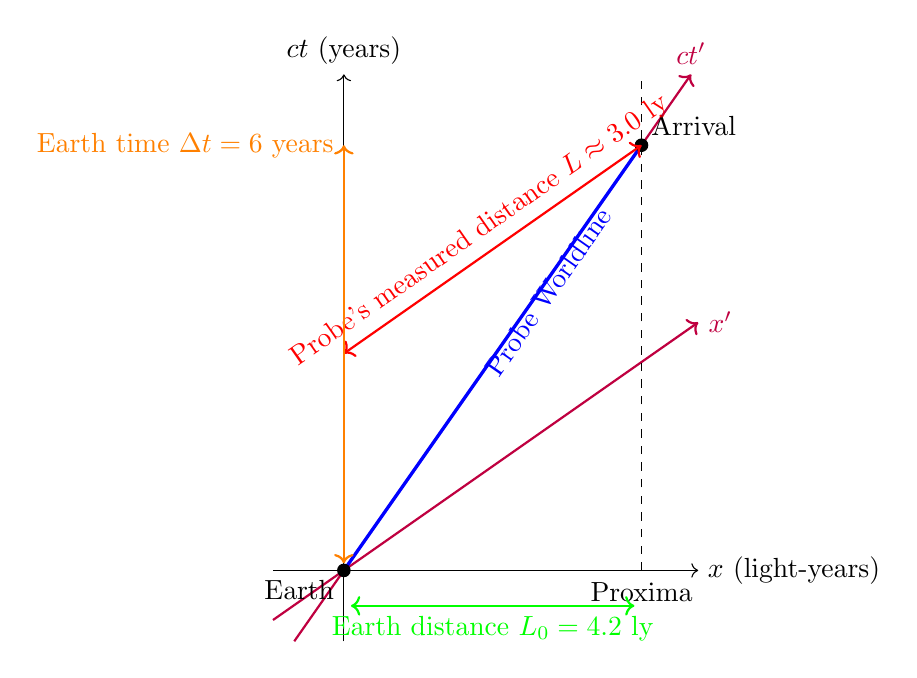
\begin{tikzpicture}[scale=0.9]
    \def\v{0.7}
    % Earth's frame (S)
    \draw[->] (-1,0) -- (5,0) node[right] {$x$ (light-years)};
    \draw[->] (0,-1) -- (0,7) node[above] {$ct$ (years)};
    
    % Probe's frame (S')
    \draw[->, purple, thick] (-1, -1*\v) -- (5, 5*\v) node[right] {$x'$};
    \draw[->, purple, thick] (-1*\v, -1) -- (7*\v, 7) node[above] {$ct'$};
    
    % Worldlines
    \draw[blue, very thick] (0,0) -- (4.2, 6); % Probe's worldline
    \draw[black, dashed] (4.2, 0) -- (4.2, 7); % Proxima Centauri's worldline
    \node[blue, anchor=south east, rotate=55, inner sep=0pt] at (3.8, 5.0) {Probe Worldline};
    \filldraw[black] (0,0) circle (2.5pt) node[below left, black] {Earth};
    \filldraw[black] (4.2, 6) circle (2.5pt) node[anchor=south west] {Arrival};
    \node at (4.2, -0.3) {Proxima};
    
    % Line of simultaneity for probe at arrival to measure contracted length
    \coordinate (ArrivalEvent) at (4.2, 6);
    \coordinate (SimultaneousOnEarthWorldline) at (0, 6 - \v * 4.2);
    \draw[<->, red, thick] (SimultaneousOnEarthWorldline) -- (ArrivalEvent) node[midway, above, sloped] {Probe's measured distance $L \approx 3.0$ ly};
    
    % Time measurement in Earth Frame
    \draw[<->, orange, thick] (0,0.1) -- (0,6) node[above, left] {Earth time $\Delta t = 6$ years};
    
    % Length measurement in Earth Frame
    \draw[<->, green, thick] (0.1, -0.5) -- (4.1, -0.5) node[midway, below] {Earth distance $L_0 = 4.2$ ly};
\end{tikzpicture}
\caption{Spacetime diagram for the probe's journey. The black axes represent the Earth's frame (S), while the purple axes represent the probe's moving frame (S'). $L_0$ is the distance in the Earth frame. $L$ (red line) is the length-contracted distance as measured simultaneously in the probe's frame at the moment of arrival.}
\end{figure}

\newpage
\subsection{Problem 2: The Satellite Explosions}
\textbf{Question:} \textit{In an observer's inertial frame S, two satellites explode. The first explosion (E1) occurs at the origin ($x_1=0$) at $t_1=0$. The second explosion (E2) occurs at position $x_2=600$ km at time $t_2=1.0$ ms. An astronaut in a spaceship is moving along the positive x-axis at speed $v$. For what range of speeds $v$ will the astronaut observe the second explosion (E2) to have occurred before the first explosion (E1)?}
\vspace{1em}

We want to find the velocity $v$ of a frame S' such that the time of the second event, $t'_2$, is less than the time of the first event, $t'_1$.
The Lorentz transformation for time is:
$$t' = \gamma \left(t - \frac{vx}{c^2}\right)$$
For the two events:
\begin{itemize}
    \item $t'_1 = \gamma (t_1 - \frac{vx_1}{c^2}) = \gamma (0 - 0) = 0$
    \item $t'_2 = \gamma (t_2 - \frac{vx_2}{c^2})$
\end{itemize}
The condition for the astronaut to see E2 before E1 is $t'_2 < t'_1$:
$$\gamma \left(t_2 - \frac{vx_2}{c^2}\right) < 0$$
Since $\gamma$ is always positive, we can divide by it:
$$t_2 - \frac{vx_2}{c^2} < 0 \implies t_2 < \frac{vx_2}{c^2}$$
Now, we solve for the speed $v$:
$$v > \frac{c^2 t_2}{x_2}$$
Let's plug in the values. First, convert to SI units:
$x_2 = 600 \text{ km} = 6 \times 10^5$ m.
$t_2 = 1.0 \text{ ms} = 1 \times 10^{-3}$ s.
$$v > \frac{(3 \times 10^8 \text{ m/s})^2 (1 \times 10^{-3} \text{ s})}{6 \times 10^5 \text{ m}}$$
$$v > \frac{9 \times 10^{16} \times 1 \times 10^{-3}}{6 \times 10^5} = \frac{9 \times 10^{13}}{6 \times 10^5} = 1.5 \times 10^8 \text{ m/s}$$
As a fraction of the speed of light:
$$v > \frac{1.5 \times 10^8 \text{ m/s}}{3 \times 10^8 \text{ m/s}} = 0.5c$$
So, the astronaut must be traveling faster than half the speed of light. The full range is $\mathbf{0.5c < v < c}$.

\newpage
\subsection{Problem 3: The Relativistic Train}
\textbf{(a)} \textit{A futuristic train, designed as a long cylinder, has a proper length of 500 m and a proper radius of 2 m. It travels along a straight track at a speed of 0.9c. What is its volume as measured by an observer standing on the ground?}
\vspace{1em}
The volume of a cylinder is $V = \pi r^2 L$. Length contraction only occurs in the direction of motion. The radius, being perpendicular to the motion, is unaffected.
First, calculate the Lorentz factor:
$$\gamma = \frac{1}{\sqrt{1 - (0.9)^2}} = \frac{1}{\sqrt{1 - 0.81}} = \frac{1}{\sqrt{0.19}} \approx 2.294$$
The contracted length $L$ is:
$$L = \frac{L_0}{\gamma} = \frac{500 \text{ m}}{2.294} \approx 218.0 \text{ m}$$
The radius $r$ remains 2 m. The volume $V'$ measured by the ground observer is:
$$V' = \pi r^2 L = \pi (2 \text{ m})^2 (218.0 \text{ m}) \approx \mathbf{2739 \textbf{ m}^3}$$
\vspace{1em}
\textbf{(b)} \textit{This train (Train A, $v_A=0.9c$) passes a shorter train (Train B, $L_{0B}=300$ m) going in the opposite direction at $v_B=-0.8c$. What is the time interval measured by a ground observer between the fronts of the trains passing and the rears of the trains passing?}
\vspace{1em}
First, find the contracted lengths in the ground frame (S). For Train A, we already have $\gamma_A \approx 2.294$ and $L_A \approx 218.0$ m.
For Train B:
$$\gamma_B = \frac{1}{\sqrt{1 - (-0.8)^2}} = \frac{1}{\sqrt{0.36}} = \frac{1}{0.6} = \frac{5}{3} \approx 1.667$$
$$L_B = \frac{L_{0B}}{\gamma_B} = \frac{300 \text{ m}}{5/3} = 180 \text{ m}$$
Let Event 1 (fronts pass) be at $(x,t)=(0,0)$.
For Event 2 (rears pass), the position of Train A's rear is $x_{RA}(t) = v_A t - L_A$.
The position of Train B's rear is $x_{RB}(t) = v_B t + L_B$.
They pass when $x_{RA}(t) = x_{RB}(t)$.
$$v_A t - L_A = v_B t + L_B \implies t(v_A - v_B) = L_A + L_B$$
$$t = \frac{L_A + L_B}{v_A - v_B} = \frac{218.0 \text{ m} + 180 \text{ m}}{0.9c - (-0.8c)} = \frac{398.0 \text{ m}}{1.7c}$$
$$t = \frac{398.0}{1.7 \times (3 \times 10^8)} = \frac{398.0}{5.1 \times 10^8} \approx \mathbf{7.80 \times 10^{-7} \textbf{ s}}$$

\newpage
\subsection{Problem 4: Proton in a Gold Nucleus}
\textbf{Question:} \textit{The radius of a gold nucleus is approximately $7.3 \times 10^{-15}$ m. Using the uncertainty principle, estimate the minimum kinetic energy (in MeV) of a proton confined within this nucleus. The rest mass of a proton is $m_p \approx 938.3$ MeV/c$^2$.}
\vspace{1em}
This problem combines the Heisenberg Uncertainty Principle with the relativistic energy-momentum relation.

\textbf{Step 1: Estimate the minimum momentum.}
The uncertainty in the proton's position can be taken as the diameter of the nucleus, $\Delta x \approx 2r$.
$$\Delta x \approx 2 \times 7.3 \times 10^{-15} \text{ m} = 1.46 \times 10^{-14} \text{ m}$$
From the uncertainty principle, the minimum momentum is approximately:
$$p \approx \frac{\hbar}{\Delta x} = \frac{1.055 \times 10^{-34} \text{ J}\cdot\text{s}}{1.46 \times 10^{-14} \text{ m}} \approx 7.226 \times 10^{-21} \text{ kg}\cdot\text{m/s}$$

\textbf{Step 2: Convert momentum to MeV/c.}
It's convenient to work in units of MeV. Let's find the value of $pc$:
$$pc = (7.226 \times 10^{-21} \text{ kg}\cdot\text{m/s}) (3 \times 10^8 \text{ m/s}) \approx 2.168 \times 10^{-12} \text{ J}$$
To convert Joules to eV, we divide by $1.602 \times 10^{-19}$ J/eV.
$$pc = \frac{2.168 \times 10^{-12} \text{ J}}{1.602 \times 10^{-19} \text{ J/eV}} \approx 1.353 \times 10^7 \text{ eV} = 13.53 \text{ MeV}$$

\textbf{Step 3: Calculate the kinetic energy.}
The relativistic energy-momentum relation is $E^2 = (pc)^2 + (m_p c^2)^2$. The kinetic energy is $K = E - m_p c^2$.
We have $pc = 13.53$ MeV and the rest energy $m_p c^2 = 938.3$ MeV.
$$E = \sqrt{(13.53 \text{ MeV})^2 + (938.3 \text{ MeV})^2}$$
$$E = \sqrt{183.1 + 880406.9} = \sqrt{880590} \approx 938.398 \text{ MeV}$$
The kinetic energy is:
$$K = E - m_p c^2 = 938.398 \text{ MeV} - 938.3 \text{ MeV} \approx \mathbf{0.098 \textbf{ MeV}}$$
Even though confined, the proton is not highly relativistic in this case.

\newpage
\subsection{Problem 5: The Unstable Tau Particle}
\textbf{Question:} \textit{The tau particle ($\tau$) is an unstable lepton with a proper mean lifetime of $2.9 \times 10^{-13}$ s. In a particle accelerator, a beam of tau particles is created and travels at a speed of 0.999c down a 100-meter flight tube.}
\vspace{1em}
\textbf{(a)} \textit{What is the mean lifetime of the tau particles as measured in the laboratory frame?}
\vspace{1em}
This is a time dilation problem. First, calculate $\gamma$:
$$\gamma = \frac{1}{\sqrt{1 - 0.999^2}} = \frac{1}{\sqrt{1 - 0.998001}} = \frac{1}{\sqrt{0.001999}} \approx 22.37$$
The dilated lifetime $\Delta t$ measured in the lab is:
$$\Delta t = \gamma \Delta t_0 = (22.37) \times (2.9 \times 10^{-13} \text{ s}) \approx \mathbf{6.49 \times 10^{-12} \textbf{ s}}$$

\textbf{(b)} \textit{What is the average distance a tau particle travels in the lab frame before decaying?}
\vspace{1em}
Using the dilated lifetime and the particle's speed in the lab:
$$d = v \Delta t = (0.999 \times 3 \times 10^8 \text{ m/s}) \times (6.49 \times 10^{-12} \text{ s}) \approx 0.00194 \text{ m} = \mathbf{1.94 \textbf{ mm}}$$

\textbf{(c)} \textit{From the tau particle's reference frame, how long is the flight tube?}
\vspace{1em}
In the tau's frame, the flight tube is moving towards it and is length-contracted:
$$L = \frac{L_0}{\gamma} = \frac{100 \text{ m}}{22.37} \approx \mathbf{4.47 \textbf{ m}}$$

\textbf{(d)} \textit{A pion traveling in the same direction is measured in the lab to have a speed of 0.95c. What is the pion's speed as measured from the reference frame of a tau particle?}
\vspace{1em}
We use the relativistic velocity addition formula.
Let the lab frame be S. The tau's frame is S'.
The velocity of S' relative to S is $v = 0.999c$.
The velocity of the pion in S is $u = 0.95c$.
The velocity of the pion in S' ($u'$) is:
$$u' = \frac{u - v}{1 - \frac{uv}{c^2}} = \frac{0.95c - 0.999c}{1 - (0.95)(0.999)} = \frac{-0.049c}{1 - 0.94905} = \frac{-0.049c}{0.05095} \approx \mathbf{-0.962c}$$
The negative sign indicates that from the tau's perspective, the pion is moving backwards, as expected since the tau is faster.

\newpage
\subsection{Problem 6: Events on a Starship}
\textbf{(a)} \textit{An event occurs at the front of a starship at $x=150$ m, $t=1.0 \mu$s. A second event occurs at the back of the starship at $x=-150$ m, $t=1.0 \mu$s, all in the Earth's frame S. The starship is moving at 0.6c along the x-axis.}
\vspace{1em}
\textbf{(i)} \textit{What is the time interval between these events as measured by a clock on the starship (frame S')?}
\vspace{1em}
In the Earth frame, the events are simultaneous ($\Delta t = 0$), but separated in space ($\Delta x = -300$ m). We use the Lorentz transformation for time for each event.
$\gamma = 1/\sqrt{1-0.6^2} = 1/\sqrt{0.64} = 1/0.8 = 1.25$.
Event 1 (front): $t'_1 = \gamma(t_1 - \frac{vx_1}{c^2}) = 1.25(10^{-6} - \frac{0.6c(150)}{c^2}) = 1.25(10^{-6} - \frac{90}{3 \times 10^8}) = 1.25(10^{-6} - 0.3 \times 10^{-6}) = 0.875 \mu s$.
Event 2 (back): $t'_2 = \gamma(t_2 - \frac{vx_2}{c^2}) = 1.25(10^{-6} - \frac{0.6c(-150)}{c^2}) = 1.25(10^{-6} + \frac{90}{3 \times 10^8}) = 1.25(10^{-6} + 0.3 \times 10^{-6}) = 1.625 \mu s$.
The time interval is $\Delta t' = t'_2 - t'_1 = 1.625 - 0.875 = \mathbf{0.75 \mu s}$.
In the ship's frame, the event at the back happens later. This is the relativity of simultaneity.

\textbf{(ii)} \textit{In which frame S'' is the spatial separation between the events zero?}
\vspace{1em}
For the spatial separation between two events to be zero, the frame S'' must be moving at a velocity $v$ such that $\Delta x'' = \gamma(\Delta x - v\Delta t)=0$.
Here, $\Delta x = x_2 - x_1 = -150 - 150 = -300$ m.
The time separation is $\Delta t = t_2 - t_1 = 1.0\mu s - 1.0\mu s = 0$.
The equation becomes $\gamma(\Delta x - v \cdot 0) = \gamma \Delta x = 0$. This would require $\Delta x = 0$, but it is -300 m. Therefore, there is \textbf{no inertial frame} where these two simultaneous (in S) events can occur at the same location. This type of interval is called "space-like".

\subsection{Problem 7: Laser Ranging a Distant Probe}
\textbf{Question:} \textit{A space probe of proper length $L_0=200$ m travels away from a space station with uniform velocity. The station sends a laser pulse towards the probe. The pulse reflects off a mirror at the probe's tail, and the reflection is received back at the station 400 seconds after the initial pulse was sent. A second pulse, sent moments later, reflects off a mirror at the probe's nose. This second reflection arrives back at the station $2.0 \mu$s after the first one. (Note: The value has been chosen to ensure a physical solution).}
\vspace{1em}
\textbf{(a)} \textit{Using the simplified model where the round-trip time is approximately twice the one-way time, how far was the probe's tail from the station when the first pulse struck it?}
\vspace{1em}
This is a standard simplification for such problems. The time for the pulse to reach the probe is taken as half the total round-trip time.
Time to reach probe: $t_1 = T_1/2 = 400 \text{ s} / 2 = 200$ s.
Distance at that instant: $d = c \times t_1 = (3 \times 10^8 \text{ m/s}) \times 200 \text{ s} = \mathbf{6.0 \times 10^{10} \textbf{ m}}$.

\textbf{(b)} \textit{What is the probe's velocity, v?}
\vspace{1em}
The difference in arrival times of the reflected pulses is $\delta T = 2.0 \mu$s. The time difference between the pulse hitting the tail and the nose, in the station frame, is modeled as $\Delta t_{station} = \delta T / 2 = 1.0 \mu$s.
This time difference arises because the light must travel the contracted length of the probe plus the distance the probe moves in that time.
$$c \Delta t_{station} = L + v \Delta t_{station} = \frac{L_0}{\gamma} + v \Delta t_{station}$$
Solving this for $v/c$ gives the formula:
$$\frac{v}{c} = \frac{(c\Delta t_{station})^2 - L_0^2}{(c\Delta t_{station})^2 + L_0^2}$$
Let's find the values:
$L_0 = 200$ m.
$c\Delta t_{station} = (3 \times 10^8 \text{ m/s}) \times (1.0 \times 10^{-6} \text{ s}) = 300$ m.
$$\frac{v}{c} = \frac{(300)^2 - (200)^2}{(300)^2 + (200)^2} = \frac{90000 - 40000}{90000 + 40000} = \frac{50000}{130000} \approx 0.385$$
The probe's velocity is $\mathbf{v \approx 0.385c}$.

\end{document}